\chapter{Background}

% Introduce what is planning under uncertainty
Planning and reasoning under uncertainty is central to robotic and artificial intelligence research and has 
been an active area of research for decades. It is an umbrella term which touches a
wide spectrum of fields: \textit{economics}, \textit{psychology}, \textit{cognitive science}, \textit{neuroscience},
\textit{robotics} and \textit{artificial intelligence}. The work in this thesis relies on results  and assumptions 
made in cognitive and neuroscience with respect to our beliefs and how we act given them. We complement 
these results by introducing them in a new light to the field of robotics and demonstrate how the human reasoning and belief system 
can be used in situations where the state space is partially observable. The second main theme our work builds on is 
state space estimation. The third component acting given uncertainty in robotics. We make use of results from all 
three fields. We provide a background overview of acting under uncertainty and situate our work within the state of the 
art.

This chapter unfolds as follows: 



\section{Decisions under Uncertainty}
% What is the the reasoning under uncertainty planning problem
% What are all the assumptions which can be made regading the belief

In this section we introduce and frame the problem we seek to solve in generic 
terms. We are concerned with finding a sequence of actions which will lead to the successful 
outcome of a problem being considered; this is the most generic definition. 

There are two key attributes which can make this problem difficult: stochastic actions and latent states. Stochastic 
actions, when applied in the same state will not always result int the same outcome. This type of uncertainty 
can arise from many sources; the outcome of chaotic actions are impossible to predict with certainty, 
think of throwing a die or flipping a coin; In outdoor robotics the terrain might lead to slippage, causing 
the robot to skid or underwater currents might drastically offset the position of an UAV; In articulated 
robots the friction between joints can accumulate to a large error in the end-effector position (especially true 
for cable driven robots). 
The second source of uncertainty is when the underlying state is partially known, in the sense that we do not 
have all the necessary information to reliably determine the state beyond reasonable doubt. In robotics this 
uncertainty can arise from inadequate or noisy sensors. If the environmental conditions in which the robot 
is located is humid, misty or dark. It can make it difficult for the robot to ascertain its position and 
to plan how to achieve a given objective.

The uncertainty of the state and actions have to be quantified. The predominant approach 
is to  represent them by probabilities. For instance the application of a forward action (for a wheeled robot) 
will result in a new position further ahead and a position to the right (due to slippage) with some probability.
An observation through the robots sensors will result in probability distribution over the robots probable location.
Given this quantification of action and observation uncertainty in terms of a probability distribution over the state, 
the agent must now take actions towards accomplishing its goal. To take a decision the agent must assign a utility 
to the outcome of his actions. The utility is to indicate a preference over the outcomes and when combined with 
probabilities leads to decision theory. 

\subsection{Decision theory}

The central question of decision theory is; \textit{how do people take decisions when faced with uncertain outcomes ?} Interest 
in such questions were typically centred around economical questions such as deciding what should be an appropriate 
investment or wager for a particular gamble. It was noted that the expected monitory outcome of a gamble as a mean of basing a decision, 
would often lead to a course of action which contradicts common sense. A famous example is the St. Petersburg paradox. Daniel Bernoulli 
proposed a solution to the problem by introducing the notion of a \textit{utility} function in which he claimed that people should base 
their decision on the expected utility instead of solely the monetary outcomes of the gamble.

\begin{quote}
  \onehalfspacing% <--- Local line spacing
  ``...the value of an item must not be based on its price, but rather on the utility it yields."\par\raggedleft--- \textup{Daniel Bernoulli},\cite{Bernoulli1954}
\end{quote}

The introduction of a utility function takes into account that the net worth of a person will influence their decision since they weigh
the gain differently. The utility function introduced by Bernoulli was the logarithm of the monetary 
outcome $x\in \{5\$,10\$,25\$\}$ weighted by their probability $p(x)$ which results in an expected utility, Equation \ref{eq:exp_utility}.
\begin{equation}\label{eq:exp_utility}
  U(x) = \displaystyle \mathop{\mathbb{E}}_{x \sim p(x)} \{ u(x) \} = \sum_{x\in X} p(x) \underbrace{\log(x)}_{u(x)}
\end{equation}

Different utility functions characterise different levels of risk. When the it is concave as it for Bernoulli's utility function
the person will be \textbf{risk-averse}. Risk-averse means that a gambler would prefer the utility of a sure outcome instead of 
taking a gamble who's expected utility is the same as the one of the sure outcome. 
This was the first introduction of a utility function.
It is later in 1944 that von Neumann and Morgenstern (\cite{VonNeumann1944}) axiomised Bernoulli's utility function 
and proved that if a decision maker has a preference over a set of lotteries\footnote{the term lottery refers 
to a probability distribution in the original text.} which satisfy four axioms
(completeness, transitivity, continuity, independence) then there exists a utility function who's expectation 
preserves this preference.
An agent whose decisions can be shown to maximise the vNM expected utility are said to be \textbf{rational} 
and otherwise \textbf{irrational}. This is the theoretical basis of most economic theory, it is
a \textbf{normative} model of how people should behave given uncertainty. 
A drawback to the vNM theory of rationality is that it lacks the descriptive power to model peoples actual 
decisions. It predicts that when we are presented with a choice with two different lotteries we will chose 
the lottery which yields the maximum expected utility. There notable human studies ([citation]) which consistently 
demonstrate that we do not always act as a vNM agent.  
Decision Theory models which try to describe how we behave and not how we should behave are known as prescriptive 
models, (see (\ref{sec:prospect_theory}) and the prospect model (\cite{Kahneman79prospecttheory})).

%How is the uncertainty quantified ? Answer: probability theory
%How does the agent make a decision ? He must assigned a preference to the outcome of various actions
%Utility theory and combined with probability lead to decision theory.

% Speak about the historical context of plannig un
% Uncertainty and rational actions


% vNM theorem is limited to evaluation options that come with an 
% objective probability distribution over outcomes.
% a situation decision theoriests and economists often describe 
% as ''choice under risk``

% The utility function represents the agents desires.
% so the probability function represents her beliefs.
% The theories are referred to collectively as subjective expected utility (SEU).

% How is decision theory used in robotics ?


\subsection{Beliefs \& desires}

% POMDPs provide a rich framework for sequential decision-making under uncertainty in stochastic domains.
% Solving a POMDP is often intractable.

%\begin{enumerate}
% \item Decision theory
% \item Markov Decision Process
% \item Partially Observable Markov Decision Process
%\end{enumerate}

%\begin{table}
%\begin{center}
%\renewcommand{\arraystretch}{1.5}
%\begin{tabular}{ l|l} 
%\hline
%    \textbf{Notation} 		& \textbf{Definition} \\ \hline\hline
%    $x_t \in \mathbb{R}^3$ 	& Cartesian state space position of the agent.\\
%    $y_t \in \mathbb{R}^{M}$	& Observation measurement from the agents sensors.\\
%    $u_t \in \mathbb{R}^3$	& Cartesian velocity, typically of the end-effector of the agent .\\
%\end{tabular}
%\end{center}
%\caption{Definition of common variables used.}
%\label{tab:notation}
%\end{table}

% Define box and box title style
\tikzstyle{pomdp_box}  = [draw=black, fill=blue!20, very thick,  rectangle, rounded corners, inner sep=10pt, inner ysep=20pt]
\tikzstyle{fancytitle} = [fill=white,draw= black, text=white,rounded corners=1mm,text=black]

\begin{figure}[h]
\centering
\begin{tikzpicture}
\node [pomdp_box] (box){%
    \begin{minipage}{\textwidth}
      \begin{itemize}
       \item[] \textbf{States, Actions, Observations} 
      
      \item[] \textbf{Transition function:} $\mathbf{p(x_{t+1}|x_t,u_t)}$\\ The state transition function models the uncertainty originating from motion noise and is 
       represented by the conditional probability distribution (or likelihood) function, $p(x_{t+1}|x_t,u_t) \in \mathbb{R}$,
       which gives the probability of moving to state $x_{t+1}$ given that action $u_t$ was applied in state $x_t$. 
      
      \item[] \textbf{Observation function}: $\mathbf{p(y_t|x_t)}$\\ The observation function returns the probability 
       or likelihood of the current observing $y_t$ given a known state $x_t$. It is modelled 
       by the conditional distribution $p(y_t|x_t) \in \mathbb{R}$.
      
      \item[] \textbf{Belief:} $\mathbf{b_t(x)}$ \\
       A belief is probability distributions, $b_t(x)$, over the state space $X$ and quantifies both 
       motion and observation uncertainty. 
      
      \item[] \textbf{State space estimator:} $\mathbf{b_t(x) = \tau(b_{t-1}(x),u_{t-1},y_t)}$\\ 
       Updates a belief given a motion and observation, it makes use of both the motion and observation functions 
       defined in the POMDP. The state space estimation function, $\tau$, can be any kind of state space filter such as 
       an Extended Kalman Filter (EKF) or a Particle Filter (PF).
    
       \item[] \textbf{Reward function:} $\mathbf{R(x_t,u_t)}$\\
        The reward becomes a function of the belief $R(b_t,u_t)$ which is the expected value of the original reward 
	function $\mathbb{E}_{x_t \sim b_t}[R(x_t,u_t)]$.
       \item[] \textbf{Discount factor} $\gamma \in [0,1]$;
      \end{itemize}
    \end{minipage}
};
\node[fancytitle, right=10pt] at (box.north west) {POMDP \& \textit{belief}-MDP};
\end{tikzpicture}%
\caption{Description of the individual elements necessary to formalise a POMDP and a \textit{belief}-MDP.}
\label{fig:pomdp_tik}
\end{figure}

\section{Partially Observable Markov Decision Process}

%An important aspect of the POMDP approach is taht thre is no distinction drawn between actions taken to change 
%the state of the world and actions taken to gain information! 
%(\cite{Kaelbling98planningand})

A POMDP is a popular approach for formulating a decision making process under both motion and measurement uncertainty;
In Figure \ref{fig:pomdp_tik} we describe all of the components necessary for a POMDP.

Since the states are not observable, the agent cannot choose its actions based on the state. The explicit 
representation of the past events is typically memory expensive. Instead it is possible to summarize all relevant 
information from previous actions and observations in a probability distribution over the state space, known as the
belief state. 

Because the state space is partially observable the expected reward has to be computed for each possible history of states, actions and observations.
All approaches in the literature instead encapsulate all these possible histories into a belief state $b_t(x_t)$ which is a 
probability distribution (referred to in the POMDP literature as an information state, \textit{I}-state) over the state space $x_t$ and use this 
new state description to cast the POMDP into a \textit{belief}-MDP (states are probability distributions, beliefs). 

The new description of the problem is now in terms of belief space $<\mathcal{B},U,\tau,R,\gamma>$ where $\mathcal{B}$ is the set of 
all possible beliefs and 
The reward becomes a function of the belief $R(b_t,u_t)$ which is the expected value of the original reward 
function $\mathbb{E}_{x_t \sim b_t}[R(x_t,u_t)]$, The goal is to find an optimal action for each belief such that 
the policy $\pi(b_t,u_t)$ maximises the expected reward, Equation \ref{eq:optimal_value_f}.

\begin{align}\label{eq:optimal_value_f}
% V^{\pi^*}(b_{t-1}) &= \mathbb{E}\left[\sum\limits_{t=0}^{\infty} \gamma^{t} R(x_t,u_t) \bigg| \pi,b_{t-1}\right]\\
 V^{\pi^*}(b_{t-1}) &= \max_{u_{t-1}} \bigg[ R(b_{t-1},u_{t-1}) + \gamma \cdot \mathbb{E}_{y_t}\left[ V^{\pi}(b_t)  \right] \bigg]
\end{align}

From considering the decision belief tree of the POMDP, Figure \ref{fig:pomdp_bel_tree}, we can appreciate the complexity of the problem
of finding an optimal policy. Given a discrete set of actions and observations to update the belief $b_1$ we have to consider a time 
complexity of $\mathcal{O}(|U||Y|^T)$ where $T$ is the depth of the tree (the planning horizon). Given that we have a finite set of 
belief the complexity solving the POMDP is $\mathcal{O}(|\mathcal{B}||U||Y|^T)$. 


\begin{figure}[h]
 \centering
 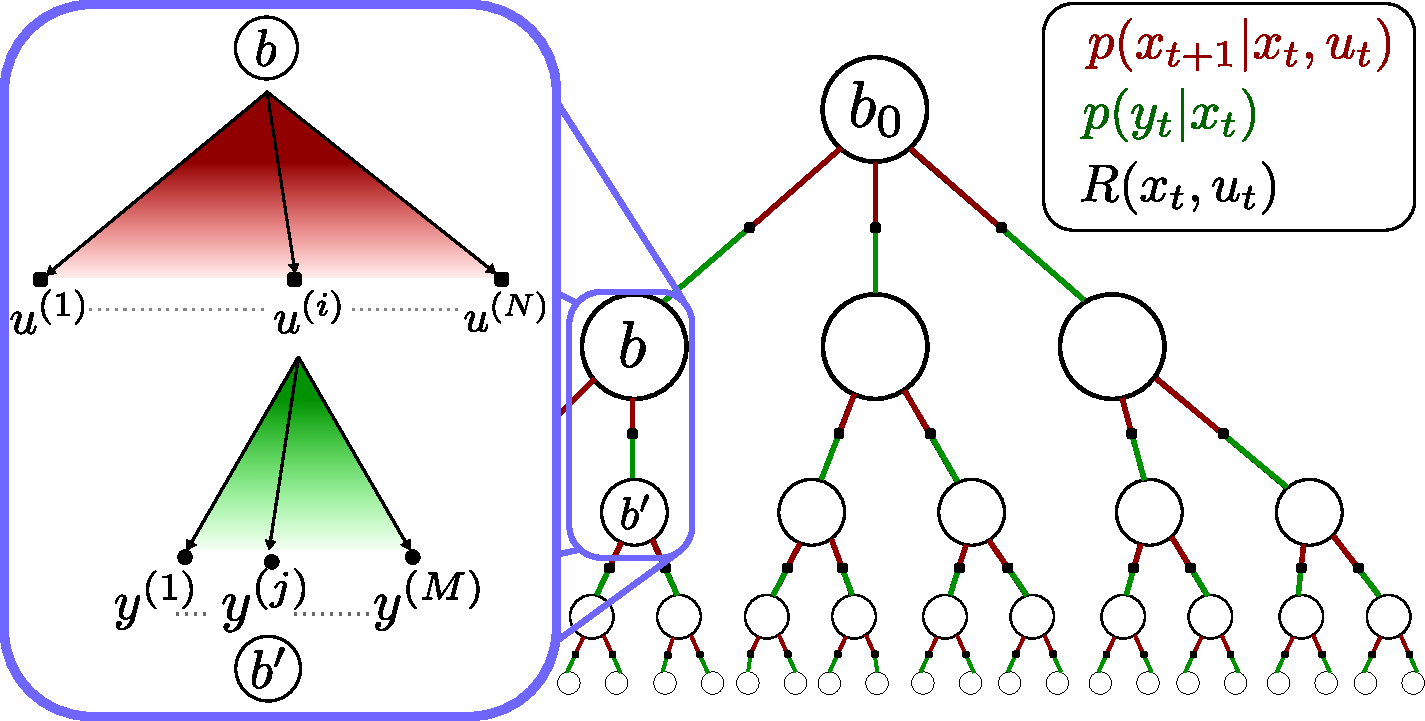
\includegraphics[width=\textwidth]{/home/guillaume/Documents/Thesis/ch2-Background/Figures/belief_tree.pdf}
  \caption{ad}
\end{figure}


\section{State of the art}

%\begin{figure}[h]
% \centering
% 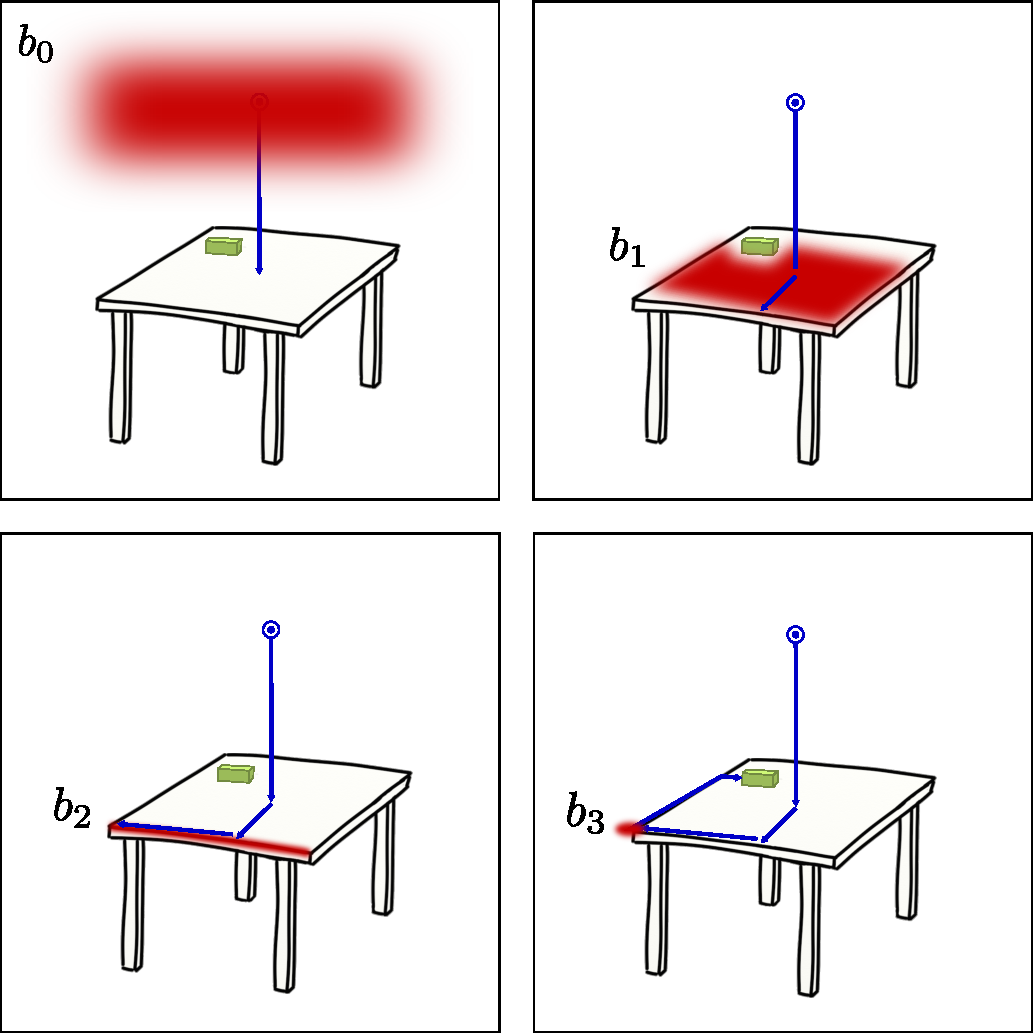
\includegraphics[width=\textwidth]{/home/guillaume/Documents/Thesis/ch2-Background/Figures/reasoning_uncertainty_concept1.pdf}
% \caption{ad}
%\end{figure}

% Standard decision theory, (no temporal aspect taken into consideration)
% Markov decision process (MDP).


% 1) POMDP
%	Based on Markove Decision Process
%	Talk about background in Optimal control and decision theor
%	Assume convex cost function, can be in feature space
%	 1.1) Approximatee POMDP
%	 1.2) MC-POMDP


% 2) Belief space (planning)
%	belief roadmap (assumption on the noise)
%
% 3)  Belief space (optimal control)
%
%
% 4) Assumptions about motion noise and observation 
%
%

% Policy search
\cite{Sol_POMDP_Policy_space_1998}

\subsubsection{Tree search}

\subsubsection{Planning}
$b = (\mu,\Sigma)$
\cite{Quadrator_2008},\cite{BelRoadMap_2009}


\subsubsection{Optimal control}
$b = (\mu,\Sigma)$
 
\cite{Erez10ascalable},
\cite{mc_update_ppomdps}, 
\cite{Platt-RSS-10}

 
% Continous

Optimal control methods represent the belief by a Gaussian function 


\cite{Bayesian_explor_exploit_2009},\cite{Spaan05icra},\cite{Thrun_2005}
 
% Sample based replanning

\cite{Rand_belief_space_replanning}
 
 
 % Online vs Offline methods
 \cite{Ross08onlineplanning}
 
 % Macro-Actions
 \cite{Macro_uncertainty_2011}

\section{Summary}




